\documentclass{article}\usepackage[]{graphicx}\usepackage[]{color}
%% maxwidth is the original width if it is less than linewidth
%% otherwise use linewidth (to make sure the graphics do not exceed the margin)
\makeatletter
\def\maxwidth{ %
  \ifdim\Gin@nat@width>\linewidth
    \linewidth
  \else
    \Gin@nat@width
  \fi
}
\makeatother

\definecolor{fgcolor}{rgb}{0.345, 0.345, 0.345}
\newcommand{\hlnum}[1]{\textcolor[rgb]{0.686,0.059,0.569}{#1}}%
\newcommand{\hlstr}[1]{\textcolor[rgb]{0.192,0.494,0.8}{#1}}%
\newcommand{\hlcom}[1]{\textcolor[rgb]{0.678,0.584,0.686}{\textit{#1}}}%
\newcommand{\hlopt}[1]{\textcolor[rgb]{0,0,0}{#1}}%
\newcommand{\hlstd}[1]{\textcolor[rgb]{0.345,0.345,0.345}{#1}}%
\newcommand{\hlkwa}[1]{\textcolor[rgb]{0.161,0.373,0.58}{\textbf{#1}}}%
\newcommand{\hlkwb}[1]{\textcolor[rgb]{0.69,0.353,0.396}{#1}}%
\newcommand{\hlkwc}[1]{\textcolor[rgb]{0.333,0.667,0.333}{#1}}%
\newcommand{\hlkwd}[1]{\textcolor[rgb]{0.737,0.353,0.396}{\textbf{#1}}}%

\usepackage{framed}
\makeatletter
\newenvironment{kframe}{%
 \def\at@end@of@kframe{}%
 \ifinner\ifhmode%
  \def\at@end@of@kframe{\end{minipage}}%
  \begin{minipage}{\columnwidth}%
 \fi\fi%
 \def\FrameCommand##1{\hskip\@totalleftmargin \hskip-\fboxsep
 \colorbox{shadecolor}{##1}\hskip-\fboxsep
     % There is no \\@totalrightmargin, so:
     \hskip-\linewidth \hskip-\@totalleftmargin \hskip\columnwidth}%
 \MakeFramed {\advance\hsize-\width
   \@totalleftmargin\z@ \linewidth\hsize
   \@setminipage}}%
 {\par\unskip\endMakeFramed%
 \at@end@of@kframe}
\makeatother

\definecolor{shadecolor}{rgb}{.97, .97, .97}
\definecolor{messagecolor}{rgb}{0, 0, 0}
\definecolor{warningcolor}{rgb}{1, 0, 1}
\definecolor{errorcolor}{rgb}{1, 0, 0}
\newenvironment{knitrout}{}{} % an empty environment to be redefined in TeX

\usepackage{alltt}
\usepackage{amscd, amssymb, amsmath, verbatim, setspace}
\usepackage[left=1.0in, right=1.0in, top=1.0in, bottom=1.0in]{geometry}
\usepackage{mathrsfs}
\usepackage{listings}


\IfFileExists{upquote.sty}{\usepackage{upquote}}{}
\begin{document}
\begin{flushright}
  Arif Ali\\
  ANLY-511 Prob. Modeling \& Stat. Computing\\
	Dec 09, 2015\\
\end{flushright}

\begin{center}
  \LARGE\textbf{Homework \#11}
\end{center}
\section*{Exercise 81}
\subsection*{Part A}
$\mu_{0}=98.6$ and $\mu_{a}>98.6$
\subsection*{Part B}
\begin{knitrout}
\definecolor{shadecolor}{rgb}{1, 1, 1}\color{fgcolor}\begin{kframe}
\begin{verbatim}
Sodor.kidstemp = c(98.0, 98.9, 99.0, 98.9, 98.8,
                   98.6, 99.1, 98.9, 98.5, 98.9, 
                   98.9, 98.4, 99.0, 99.2, 98.6, 
                   98.8, 98.9, 98.7)


pt((mean(Sodor.kidstemp)-98.6)/
  (sd(Sodor.kidstemp)/sqrt(length(Sodor.kidstemp))), 
  df = length(Sodor.kidstemp)-1, lower.tail = F)
## [1] 0.006906586
\end{verbatim}
\end{kframe}
\end{knitrout}
Since the p-value is less than 0.05, we can conlcude that the average child's temperture in Sodor is higher than normal.
\section*{extra credit 1}
\begin{knitrout}
\definecolor{shadecolor}{rgb}{1, 1, 1}\color{fgcolor}\begin{kframe}
\begin{verbatim}
Sodor.kidstemp.ci = replicate(10000, mean(sample(Sodor.kidstemp, length(Sodor.kidstemp), replace = T)))
quantile(Sodor.kidstemp.ci, c(0.05))
##       5% 
## 98.66667
\end{verbatim}
\end{kframe}
\end{knitrout}
Based on the confidence interval, we can be 95\% is between 98.65 and 98.90, which follows the idea from Exercise 81 Part B, where the p-value is highly significiant. We can, again, conclude that the average child's temperture in Sodor is higher than normal.
\section*{Exercise 82}
\subsection*{Part A}
\begin{knitrout}
\definecolor{shadecolor}{rgb}{1, 1, 1}\color{fgcolor}\begin{kframe}
\begin{verbatim}
prop.test(c(28,13),c(250,250))$conf.int
## [1] 0.008191018 0.111808982
## attr(,"conf.level")
## [1] 0.95
\end{verbatim}
\end{kframe}
\end{knitrout}
We are 95\%confident that the difference in infection between the two oxygen groups is between 0.008191018 and 0.111808982.
\subsection*{Part B}
Because there is no control group, we cannot determine whether the adding oxygen to the samples result in some sort difference (whether significant or not).
\section*{Exercise 83}
\subsection*{Part A}
Type I error: If after testing the 15 households, we get a P-value given an $\alpha$ such that we reject the null hypothesis in favor of the alternative hypothesis $\mu>10$. However, the aresenic level is still $\mu=10$. Thus, a significant amount of money could be invested to clean up arsen, even though it doesn't pose a series problem.
Type II error, the sample tests show that the level aren't elevated. Even though there is an arsenic level problem, it's dismissed. People may die due to this situation.
\subsection*{Part B}
The T-distribution will look approximately the same as using the standard normal distribution; but it will not neccesarily be the same, hence the approximation. The tails will move further away from zero than with a standard normal distribution.
\section*{extra credit 2}
\subsection*{Part A}
$H_{0}:\theta=1/2$ and $H_{A}:\theta=1/4$ and $f(x;\theta)=\theta x^{\theta-1}$

\begin{equation}
  L(\theta)=\frac{1/2x^{-1/2}}{1/4x^{-3/4}}=2x^{-1/2+3/4}=2x^{1/4}
 \end{equation}

\begin{knitrout}
\definecolor{shadecolor}{rgb}{1, 1, 1}\color{fgcolor}\begin{kframe}
\begin{verbatim}
log.likelhood = function(x){2*x^(1/4)}
curve(log.likelhood)

h0 = function(x){1/2*x^(-1/2)}
curve(h0, add = T, col = "blue")

ha = function(x){1/4*x^(-3/4)}
curve(ha, add = T, col = "red")
\end{verbatim}
\end{kframe}
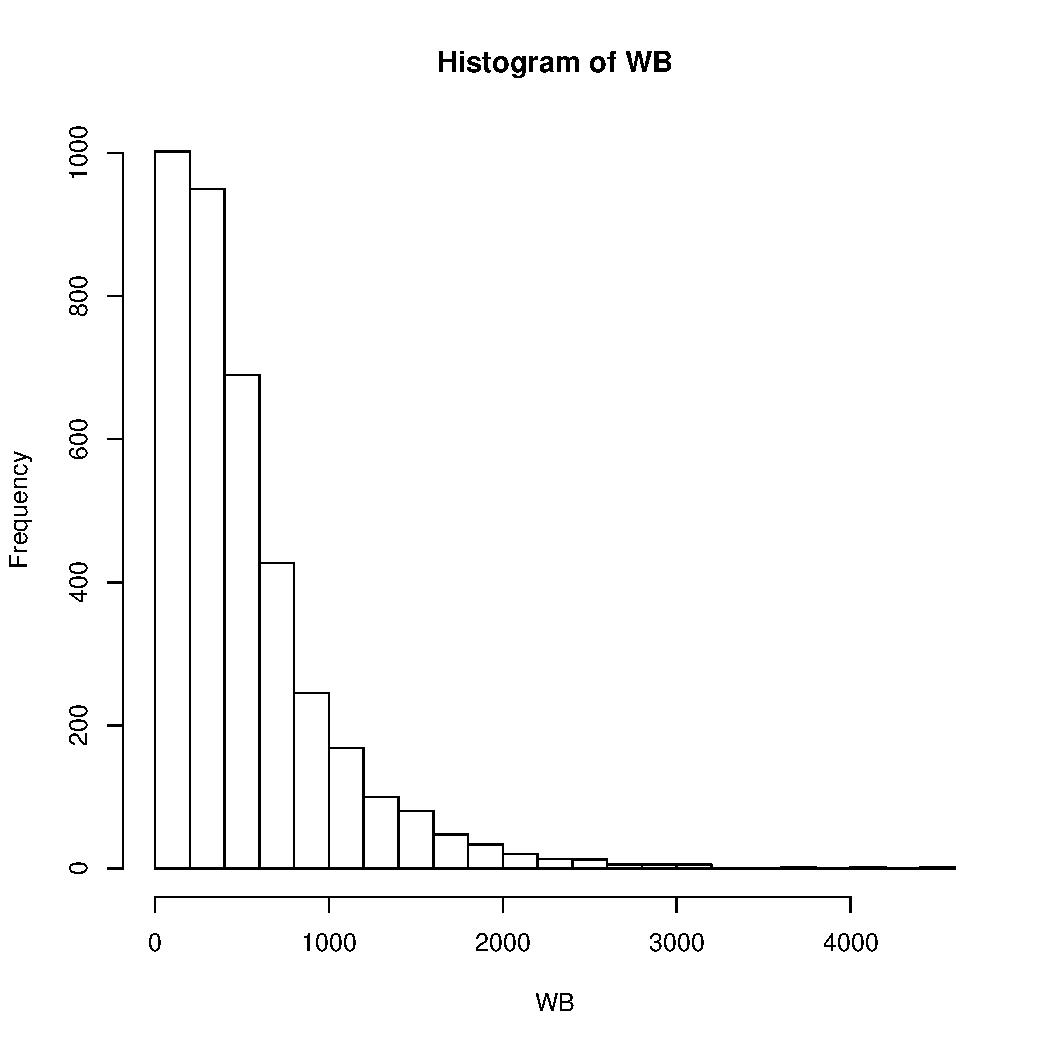
\includegraphics[width=0.33\linewidth]{figure/unnamed-chunk-5-1} 

\end{knitrout}
\begin{equation}
\int_{0}^{c}\frac{1}{2}x^{-\frac{1}{2}}dx=\Big|_{0}^{c}\sqrt{x}=0.05\implies c=(0.05)^{2}=0.0025
\end{equation}
\subsection*{Part B}
\begin{equation}
\int_{0}^{0.0025}\frac{1}{4}x^{-\frac{3}{4}}dx=\Big|_{0}^{0.0025}\sqrt[4]{x}=0.223607
\end{equation}
\section*{Exercise 84}
\subsection*{Part A}
$\mu_{y}=94$ and $\sigma_{y}=15$, $\mu_{x}=46$ and $\sigma_{x}=7$, $\rho = 0.75$

\begin{equation}
weight = 1.607143*height + 20.07142
\end{equation}
\subsection*{Part B}
\begin{knitrout}
\definecolor{shadecolor}{rgb}{1, 1, 1}\color{fgcolor}\begin{kframe}
\begin{verbatim}
1.607143*(12*5) + 20.07142
## [1] 116.5
\end{verbatim}
\end{kframe}
\end{knitrout}
\subsection*{Part C}
\begin{knitrout}
\definecolor{shadecolor}{rgb}{1, 1, 1}\color{fgcolor}\begin{kframe}
\begin{verbatim}
0.75*0.75
## [1] 0.5625
\end{verbatim}
\end{kframe}
\end{knitrout}
\section*{extra credit 3}
\subsection*{Part A}
\begin{knitrout}
\definecolor{shadecolor}{rgb}{1, 1, 1}\color{fgcolor}\begin{kframe}
\begin{verbatim}
Volleyball2009 <- read.csv("~/Dropbox/School/Georgetown/Analytics 511 Fall 2015/ChiharaHesterberg/Volleyball2009.csv")
plot(Kills~Assts, data = Volleyball2009)
\end{verbatim}
\end{kframe}
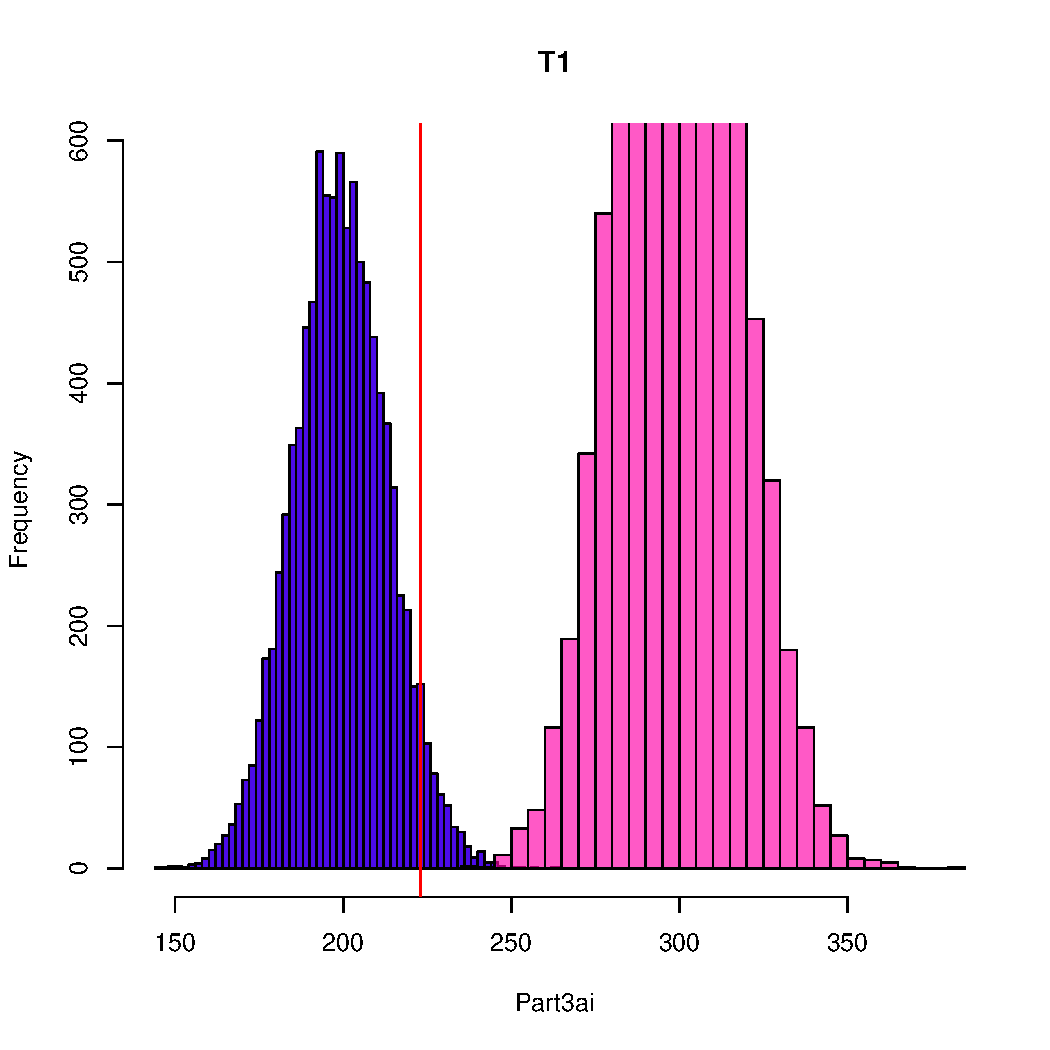
\includegraphics[width=0.33\linewidth]{figure/unnamed-chunk-8-1} 

\end{knitrout}
There seems to be a positive relationship between Kills and Assts. This is based on a pattern that could be fitted to a line with a positive slope.
\subsection*{Part B}
\begin{knitrout}
\definecolor{shadecolor}{rgb}{1, 1, 1}\color{fgcolor}\begin{kframe}
\begin{verbatim}
part_b = lm(Kills~Assts, data = Volleyball2009)
part_b$coefficients
## (Intercept)       Assts 
##   1.7362551   0.9469872
summary(part_b)$r.squared
## [1] 0.9367418
\end{verbatim}
\end{kframe}
\end{knitrout}
The slope is positive and close to one, confirming my assumptions from the scatter plot. The R Square is about very high, so a significiant amount of the variability in kills is explained via the regression.
\subsection*{Part C}
\begin{knitrout}
\definecolor{shadecolor}{rgb}{1, 1, 1}\color{fgcolor}\begin{kframe}
\begin{verbatim}
plot(Volleyball2009$Assts, resid(part_b), ylab = "Residuals")
 abline(h=0)
 
lines(smooth.spline(Volleyball2009$Assts, resid(part_b), df = 3),
col="blue") 
\end{verbatim}
\end{kframe}
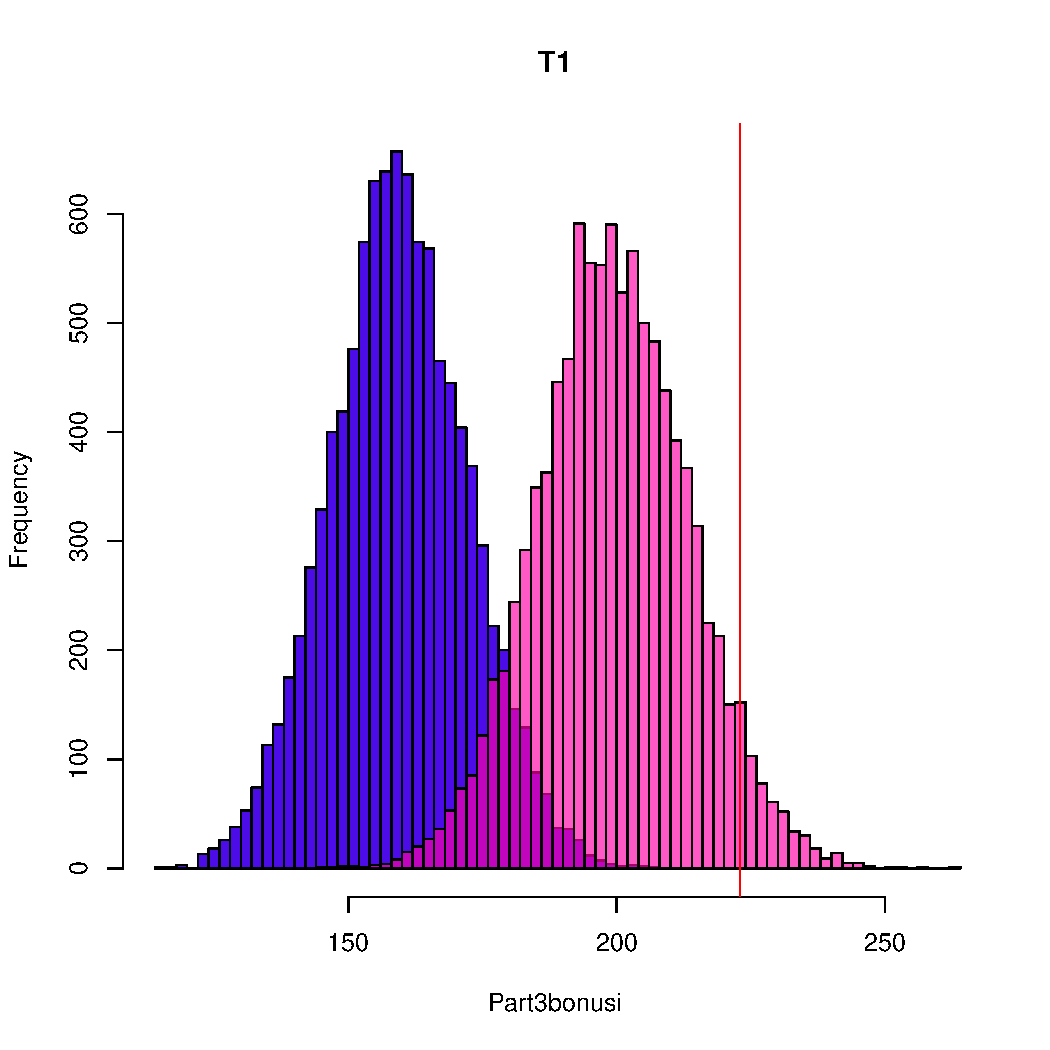
\includegraphics[width=0.33\linewidth]{figure/unnamed-chunk-10-1} 

\end{knitrout}
Based on the residuals, it seems like the straight line method is appropiate given the problem. 
\section*{Exercise 85}
\subsection*{Part A}
\begin{knitrout}
\definecolor{shadecolor}{rgb}{1, 1, 1}\color{fgcolor}\begin{kframe}
\begin{verbatim}
Maunaloa <- read.csv("~/Dropbox/School/Georgetown/Analytics 511 Fall 2015/ChiharaHesterberg/Maunaloa.csv")

plot(Level~Year, data = Maunaloa)
\end{verbatim}
\end{kframe}
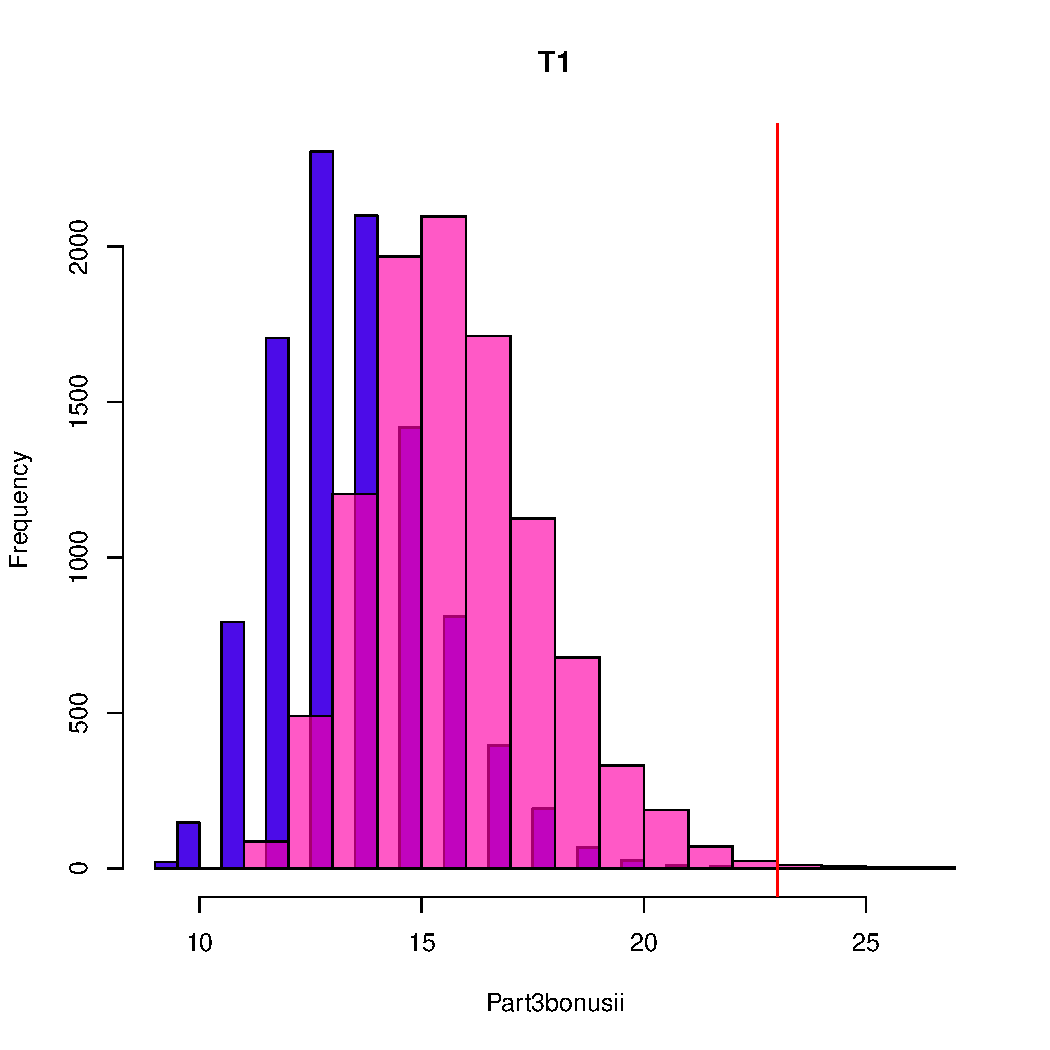
\includegraphics[width=0.33\linewidth]{figure/unnamed-chunk-11-1} 

\end{knitrout}
There seems to be a postive relationship between the Level of $CO_{2}$ and Year. This due to a positive slope of a line that could be fitted to the scatter plot. The intercept will be positive as well based on the range of Levels.
\subsection*{Part B}
\begin{knitrout}
\definecolor{shadecolor}{rgb}{1, 1, 1}\color{fgcolor}\begin{kframe}
\begin{verbatim}
Maunaloa.lm = lm(Level~Year, data = Maunaloa)
Maunaloa.lm$coefficients
##  (Intercept)         Year 
## -3279.592814     1.826403
\end{verbatim}
\end{kframe}
\end{knitrout}
\begin{equation}
Level = 1.826403*Year-3279.592814
\end{equation}
\subsection*{Part C}
\begin{knitrout}
\definecolor{shadecolor}{rgb}{1, 1, 1}\color{fgcolor}\begin{kframe}
\begin{verbatim}
plot(Maunaloa$Year,Maunaloa.lm$residuals)
\end{verbatim}
\end{kframe}
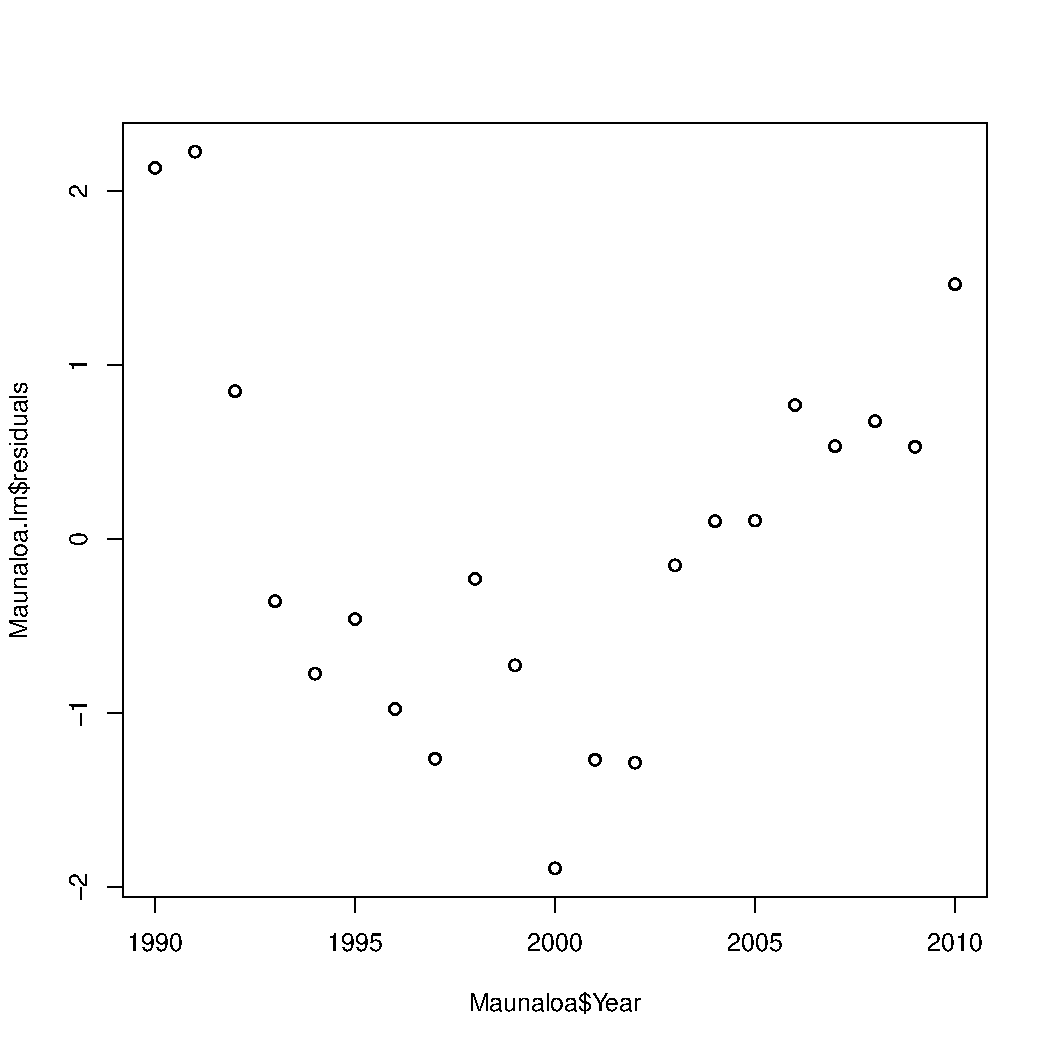
\includegraphics[width=0.33\linewidth]{figure/unnamed-chunk-13-1} 

\end{knitrout}
The residuals are very scattered, so the straight line model may not be the most appropiate measure. (The back of the book indicates it's probably serial correlation), which states that past measures affect future measurement, which makes sense because how $CO_{2}$ levels are measured.
\section*{Exercise 86}
\subsection*{Part A}
Since $X_{i}~Bern(p)$ then $Y~Bin(12, p)$
So the Probability of the type I error is:
$P(Reject H_{0}|H_{0} true) = P(\hat{p}<0.3|p=0.3 = P(k=0|p=0.3)+P(k=1|p=0.3)=(0.3)^0*(1-0.3)^{12}+\left(\begin{array}{c}
12\\
1
\end{array}\right)*(0.3)^1*(1-0.3)^{11}=0.0850250$

\subsection*{Part B}
$1 - \beta = P(Reject H_{0} | H_{A} true)=P(H_{0}\not=p| \hat{p}<p)=1-P(H_{0}=p| \hat{p}<p) = ((p)^0*(1-p)^{12}+12*(p)^1*(1-p)^{11})$
\begin{knitrout}
\definecolor{shadecolor}{rgb}{1, 1, 1}\color{fgcolor}\begin{kframe}
\begin{verbatim}
power = function(p){
  ((p)^0*(1-p)^12+12*(p)^1*(1-p)^11)
}
\end{verbatim}
\end{kframe}
\end{knitrout}
\subsection*{Part C}
\begin{knitrout}
\definecolor{shadecolor}{rgb}{1, 1, 1}\color{fgcolor}\begin{kframe}
\begin{verbatim}
p = seq(0,.3,0.01)
plot(p, power(p))
\end{verbatim}
\end{kframe}
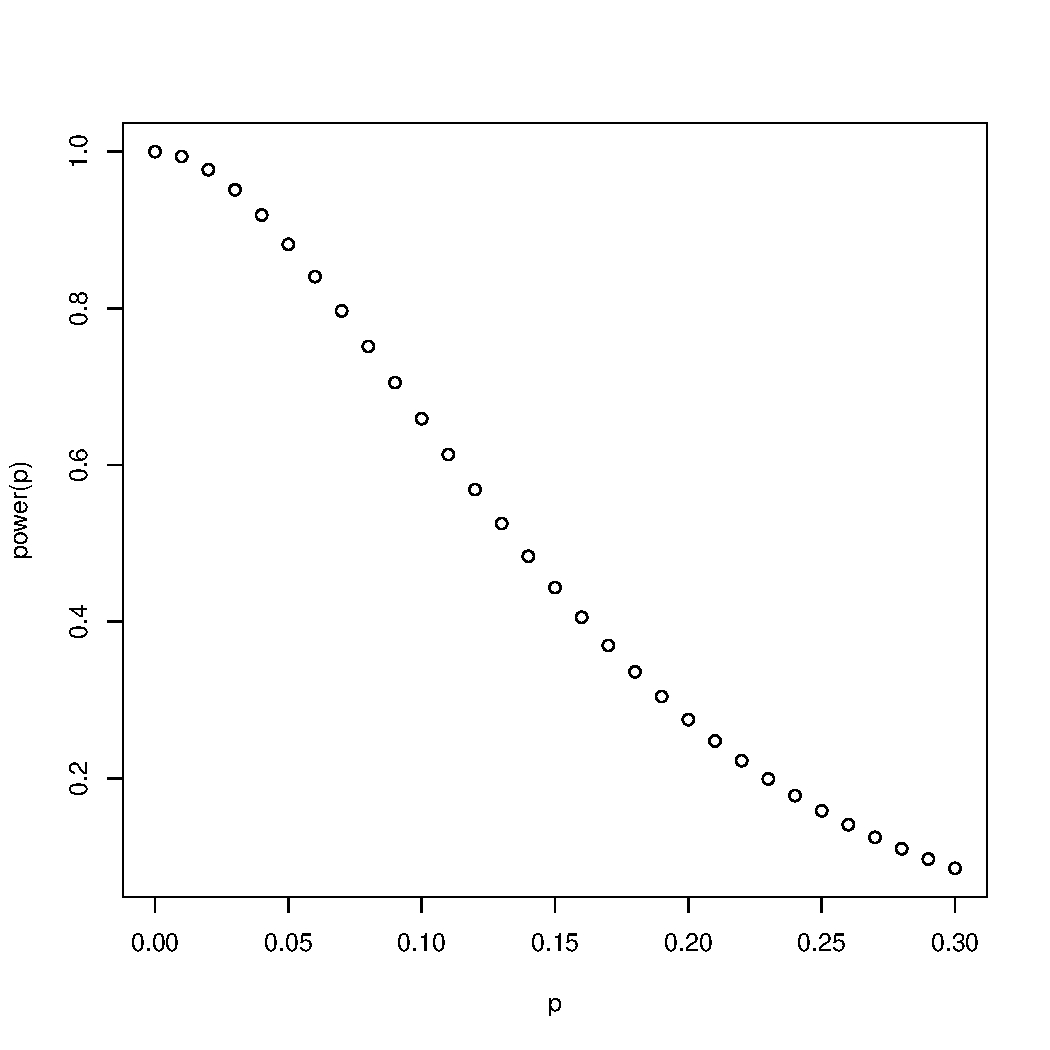
\includegraphics[width=0.33\linewidth]{figure/unnamed-chunk-15-1} 

\end{knitrout}

\section*{Exercise 87}
\subsection*{Part A}
\begin{knitrout}
\definecolor{shadecolor}{rgb}{1, 1, 1}\color{fgcolor}\begin{kframe}
\begin{verbatim}
corrExerciseA <- read.csv("~/Dropbox/School/Georgetown/Analytics 511 Fall 2015/ChiharaHesterberg/corrExerciseA.csv")
plot(Y~X, data = corrExerciseA)
\end{verbatim}
\end{kframe}
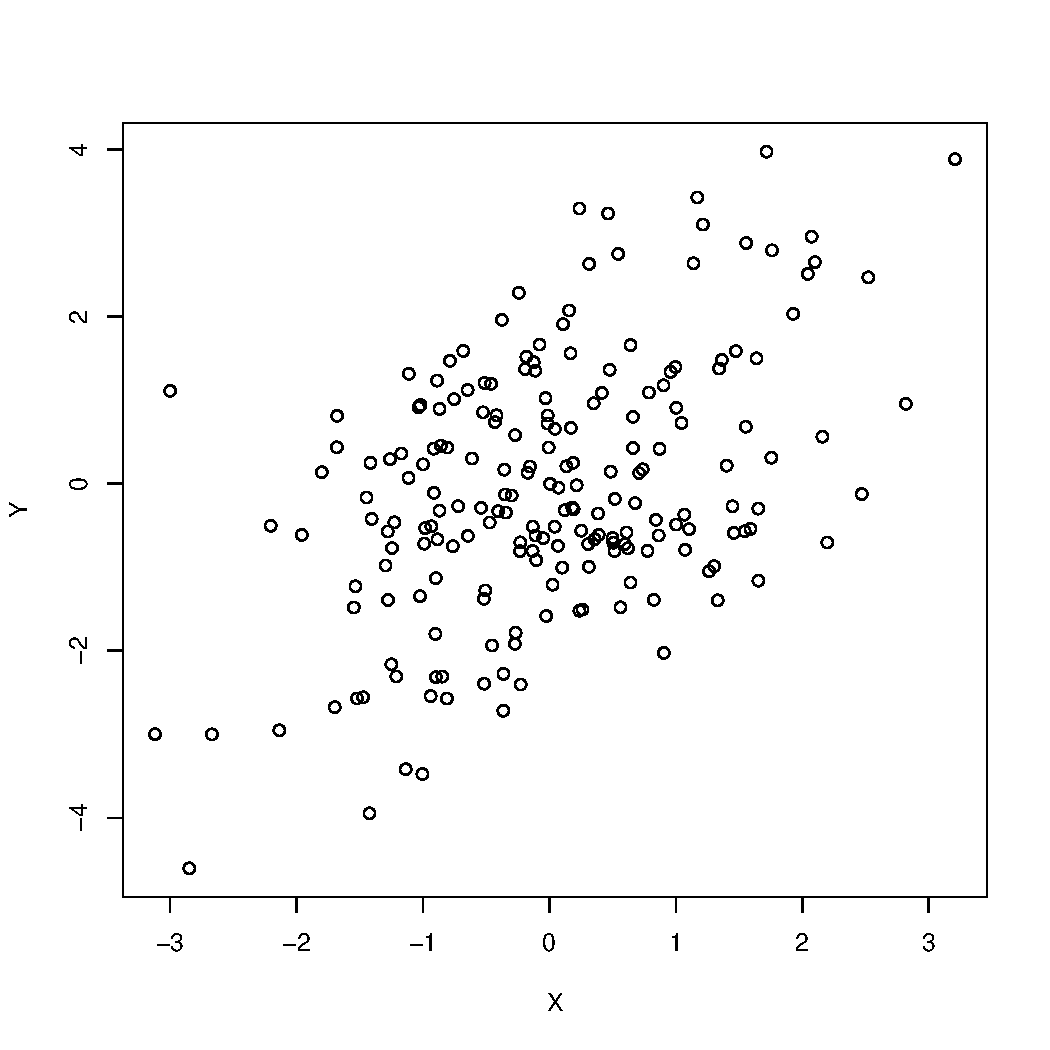
\includegraphics[width=0.33\linewidth]{figure/unnamed-chunk-16-1} 
\begin{kframe}\begin{verbatim}
cor(corrExerciseA$X, corrExerciseA$Y)
## [1] 0.4550343
\end{verbatim}
\end{kframe}
\end{knitrout}
\subsection*{Part B}
\begin{knitrout}
\definecolor{shadecolor}{rgb}{1, 1, 1}\color{fgcolor}\begin{kframe}
\begin{verbatim}
plot(Y~X, 
     data = corrExerciseA[corrExerciseA$Z=="A",],
     main = "A")

plot(Y~X, 
     data = corrExerciseA[corrExerciseA$Z=="B",],
     main = "B")
\end{verbatim}
\end{kframe}
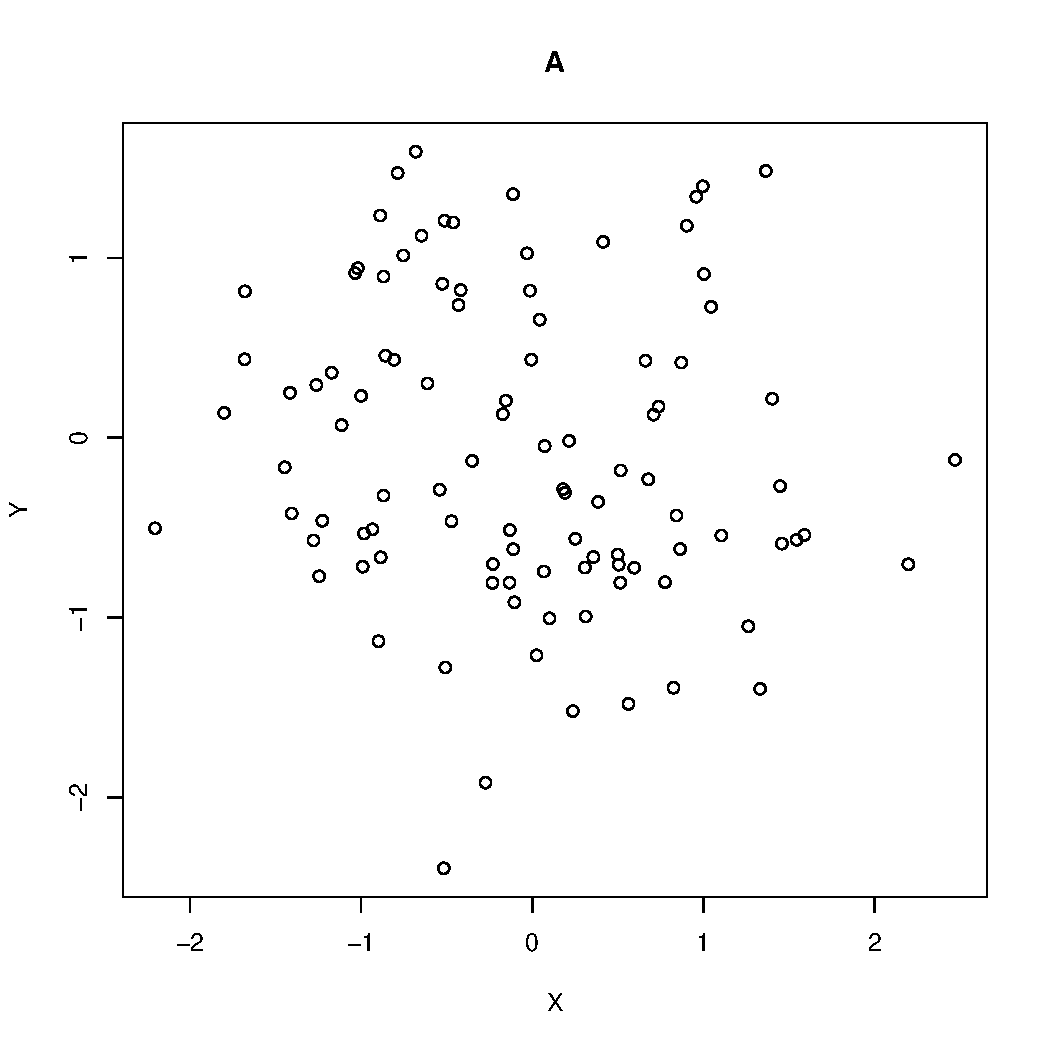
\includegraphics[width=0.33\linewidth]{figure/unnamed-chunk-17-1} 
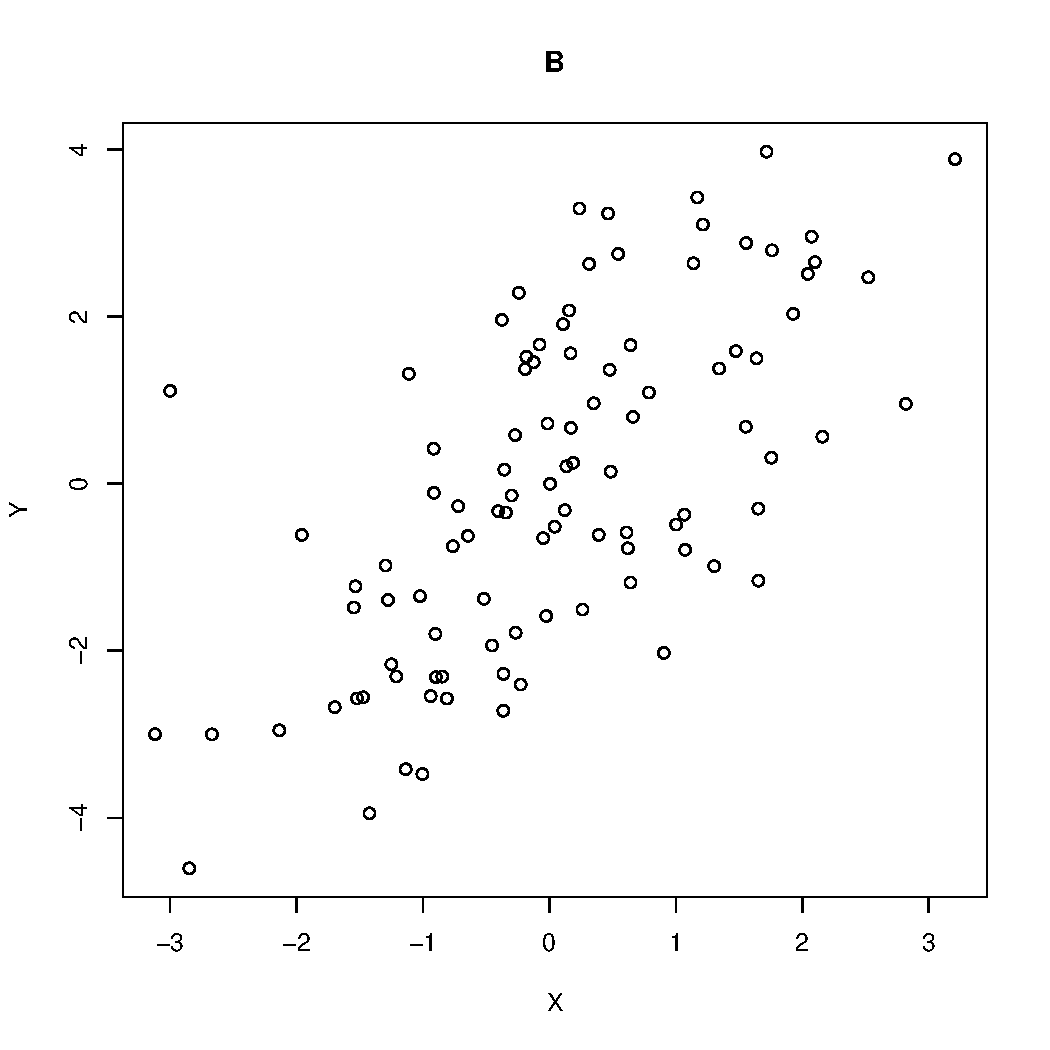
\includegraphics[width=0.33\linewidth]{figure/unnamed-chunk-17-2} 

\end{knitrout}
Plot A is trending downward, so there must be a negative relation between X and Y in subset A.
Plot B indicates a more positive relationsip between X and Y in subset B compared to subset A or overall.
\subsection*{Part C}
\begin{knitrout}
\definecolor{shadecolor}{rgb}{1, 1, 1}\color{fgcolor}\begin{kframe}
\begin{verbatim}
print("A")
## [1] "A"
cor(corrExerciseA[corrExerciseA$Z=="A","X"],
    corrExerciseA[corrExerciseA$Z=="A","Y"])
## [1] -0.1335408
print("B")
## [1] "B"
cor(corrExerciseA[corrExerciseA$Z=="B","X"],
    corrExerciseA[corrExerciseA$Z=="B","Y"])
## [1] 0.65303
\end{verbatim}
\end{kframe}
\end{knitrout}
\subsection*{Part D}
Based on the correlations, it seems that a very large positive correlation within a dataset will help mask the fact that other subsets have negative correlations. 
\section*{Exercise 88}
\subsection*{Part A (17)}
\begin{knitrout}
\definecolor{shadecolor}{rgb}{1, 1, 1}\color{fgcolor}\begin{kframe}
\begin{verbatim}
NCBirths2004 <- read.csv("~/Dropbox/School/Georgetown/Analytics 511 Fall 2015/ChiharaHesterberg/NCBirths2004.csv")
plot(Weight~Gestation, data = NCBirths2004)
\end{verbatim}
\end{kframe}
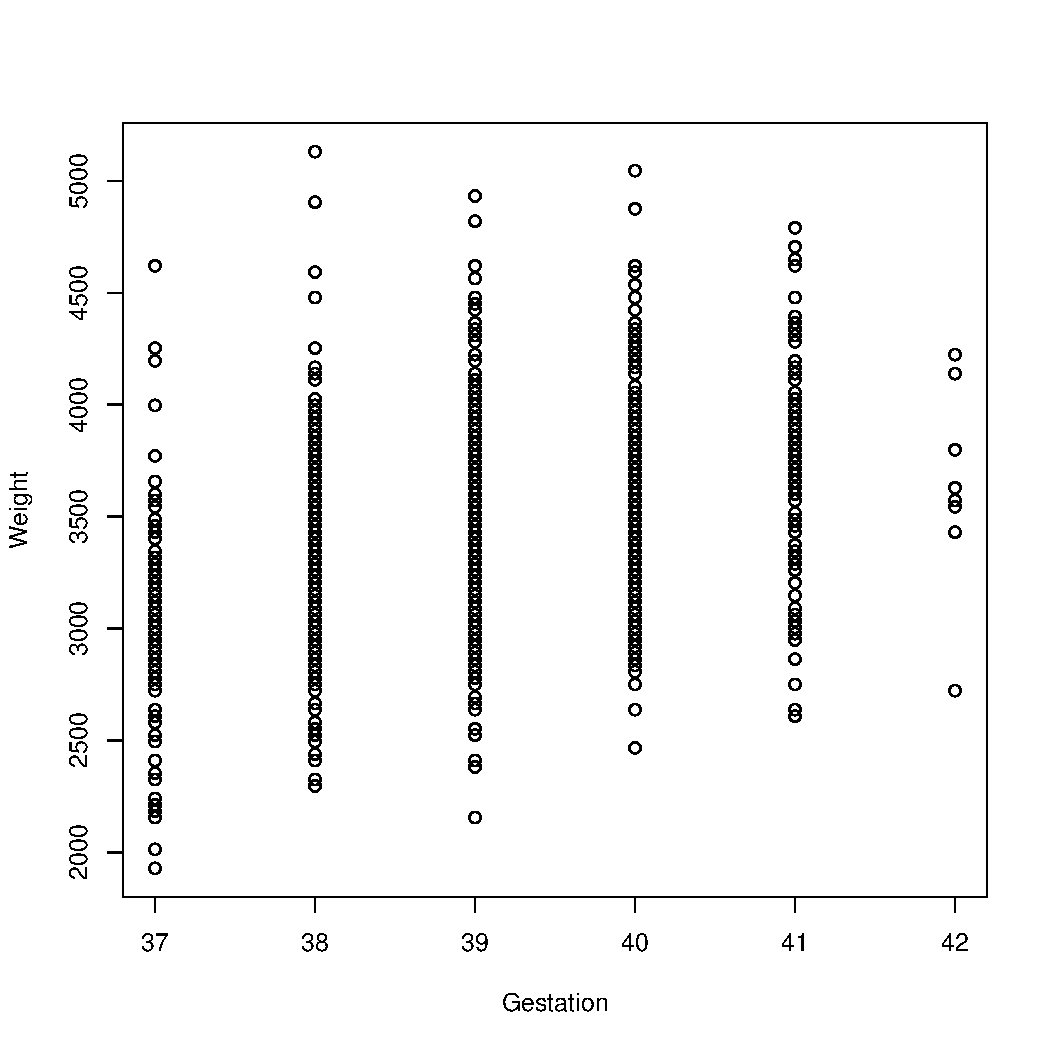
\includegraphics[width=0.33\linewidth]{figure/unnamed-chunk-19-1} 
\begin{kframe}\begin{verbatim}
cor(NCBirths2004$Weight, NCBirths2004$Gestation)
## [1] 0.3486057
\end{verbatim}
\end{kframe}
\end{knitrout}
\subsection*{Part B (17)}
\begin{knitrout}
\definecolor{shadecolor}{rgb}{1, 1, 1}\color{fgcolor}\begin{kframe}
\begin{verbatim}
part_b = lm(Weight~Gestation, data = NCBirths2004)
part_b$coefficients
## (Intercept)   Gestation 
##  -2379.6896    148.9954
\end{verbatim}
\end{kframe}
\end{knitrout}
\begin{equation}
Weight = 148.9954*Gestation - 2379.6896
\end{equation}
\subsection*{Part C (17)}
\begin{knitrout}
\definecolor{shadecolor}{rgb}{1, 1, 1}\color{fgcolor}\begin{kframe}
\begin{verbatim}
summary(part_b)$r.squared
## [1] 0.1215259
\end{verbatim}
\end{kframe}
\end{knitrout}
The slope helps indicate a postive relationship between Gestation and Weight. However, based on the $R^2$, the fact that it's small means that most of the data isn't close fitted to the line, which makes sense from the plot where the range of Weights by Gestation is spread out.
\subsection*{Part D (17)}
\begin{knitrout}
\definecolor{shadecolor}{rgb}{1, 1, 1}\color{fgcolor}\begin{kframe}
\begin{verbatim}
plot(NCBirths2004$Gestation, part_b$residuals)
\end{verbatim}
\end{kframe}
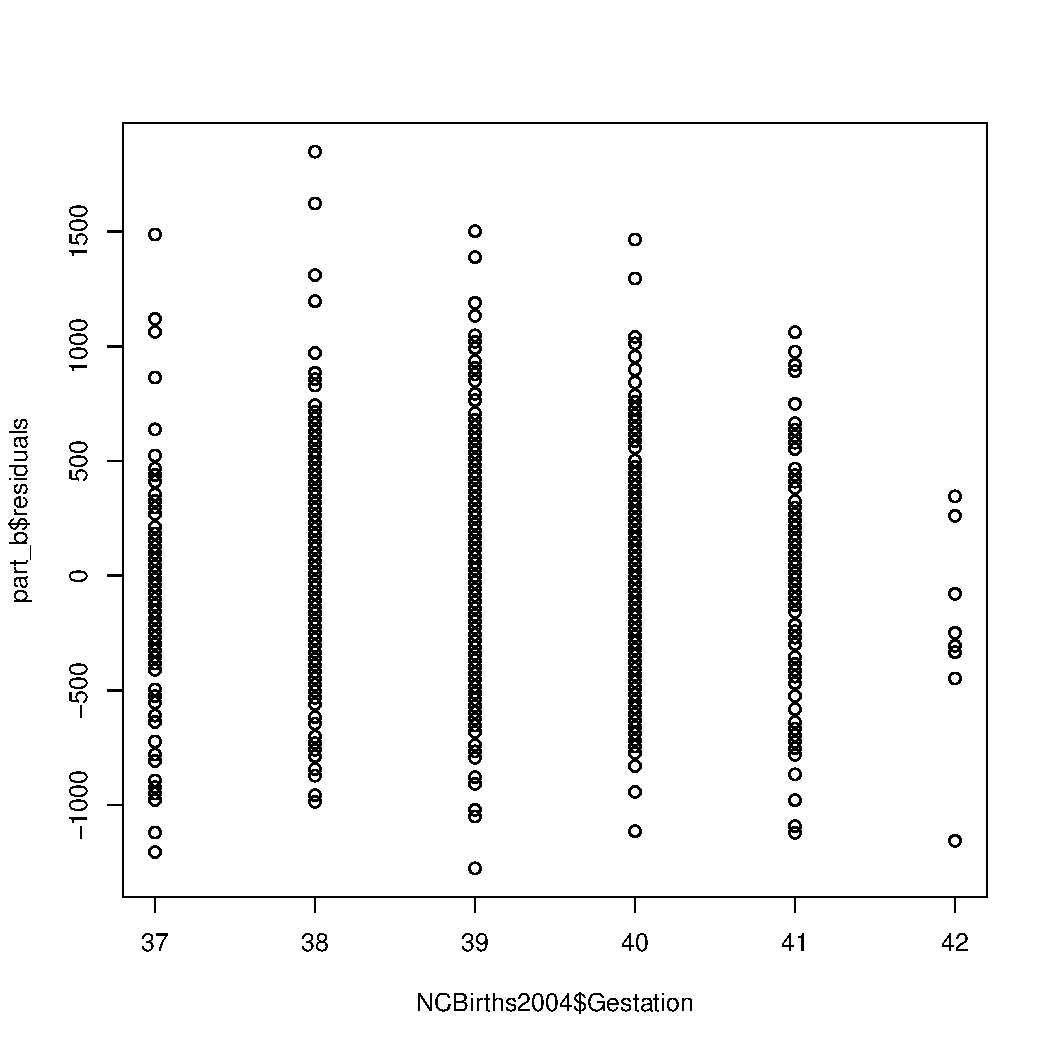
\includegraphics[width=0.33\linewidth]{figure/unnamed-chunk-22-1} 

\end{knitrout}
The residual plots looks significiantly like the plot from Part A. We need to look as each Gestation individually, because there is wide weight ranges for each period.
\subsection*{Part A (18)}
\begin{knitrout}
\definecolor{shadecolor}{rgb}{1, 1, 1}\color{fgcolor}\begin{kframe}
\begin{verbatim}
summary(part_b)
## 
## Call:
## lm(formula = Weight ~ Gestation, data = NCBirths2004)
## 
## Residuals:
##      Min       1Q   Median       3Q      Max 
## -1276.13  -312.13   -22.13   267.88  1848.87 
## 
## Coefficients:
##             Estimate Std. Error t value Pr(>|t|)    
## (Intercept) -2379.69     493.99  -4.817 1.68e-06 ***
## Gestation     149.00      12.62  11.803  < 2e-16 ***
## ---
## Signif. codes:  0 '***' 0.001 '**' 0.01 '*' 0.05 '.' 0.1 ' ' 1
## 
## Residual standard error: 457.4 on 1007 degrees of freedom
## Multiple R-squared:  0.1215,	Adjusted R-squared:  0.1207 
## F-statistic: 139.3 on 1 and 1007 DF,  p-value: < 2.2e-16
\end{verbatim}
\end{kframe}
\end{knitrout}
Estimate of $\sigma$ is 457.4.
\subsection*{Part B (18)}
\begin{knitrout}
\definecolor{shadecolor}{rgb}{1, 1, 1}\color{fgcolor}\begin{kframe}
\begin{verbatim}
summary(part_b)$coefficients[,1][2] +
  1.96*c(-1,1)*summary(part_b)$coefficients[,2][2]
## [1] 124.2529 173.7379
\end{verbatim}
\end{kframe}
\end{knitrout}

\section*{extra credit 4}
\begin{knitrout}
\definecolor{shadecolor}{rgb}{1, 1, 1}\color{fgcolor}\begin{kframe}
\begin{verbatim}
Alelager <- read.csv("~/Dropbox/School/Georgetown/Analytics 511 Fall 2015/ChiharaHesterberg/Alelager.csv")
cor(Alelager$Alcohol, Alelager$Calories)
## [1] 0.5371458
Alesampler = function(){
  index = sample(1:nrow(Alelager), nrow(Alelager), replace = T)
  Alelager.bool = Alelager[index, ]
  cor(Alelager.bool$Alcohol, Alelager.bool$Calories)
}


Alelager.bootstrap.ci = replicate(10000, Alesampler())
                        
quantile(Alelager.bootstrap.ci, c(0.025, .975))
##      2.5%     97.5% 
## 0.3699625 0.7498074
\end{verbatim}
\end{kframe}
\end{knitrout}

\section*{extra credit 5}
\subsection*{Part A}
\begin{knitrout}
\definecolor{shadecolor}{rgb}{1, 1, 1}\color{fgcolor}\begin{kframe}
\begin{verbatim}
FlightDelays <- read.csv("~/Dropbox/School/Georgetown/Analytics 511 Fall 2015/ChiharaHesterberg/FlightDelays.csv")
FlightDelays$Carrier = as.character(FlightDelays$Carrier)
boxplot(Delay~Carrier, data = FlightDelays)
hist(FlightDelays$Delay[FlightDelays$Carrier=="AA"])
hist(FlightDelays$Delay[FlightDelays$Carrier=="UA"])
qqnorm(FlightDelays$Delay[FlightDelays$Carrier=="AA"])
qqnorm(FlightDelays$Delay[FlightDelays$Carrier=="UA"])
\end{verbatim}
\end{kframe}
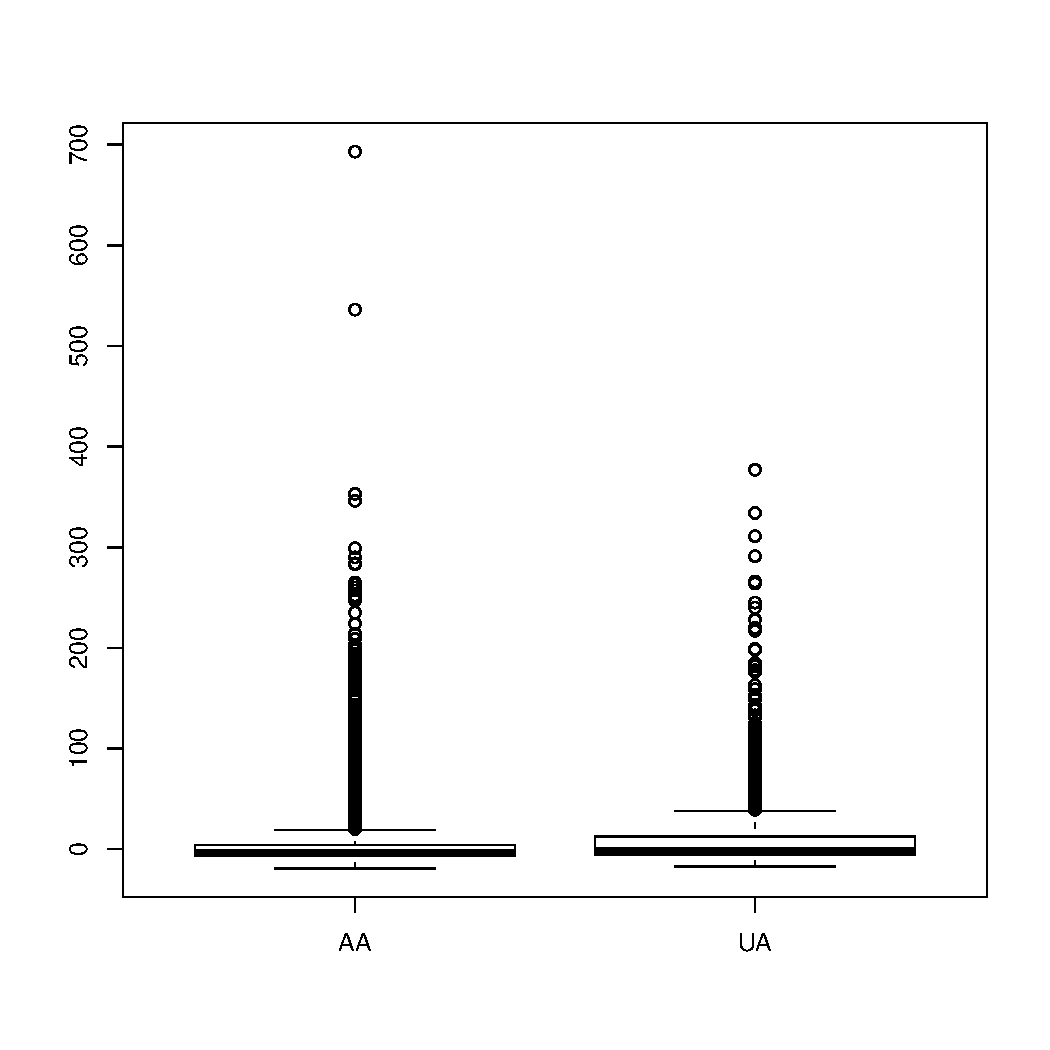
\includegraphics[width=0.33\linewidth]{figure/unnamed-chunk-26-1} 
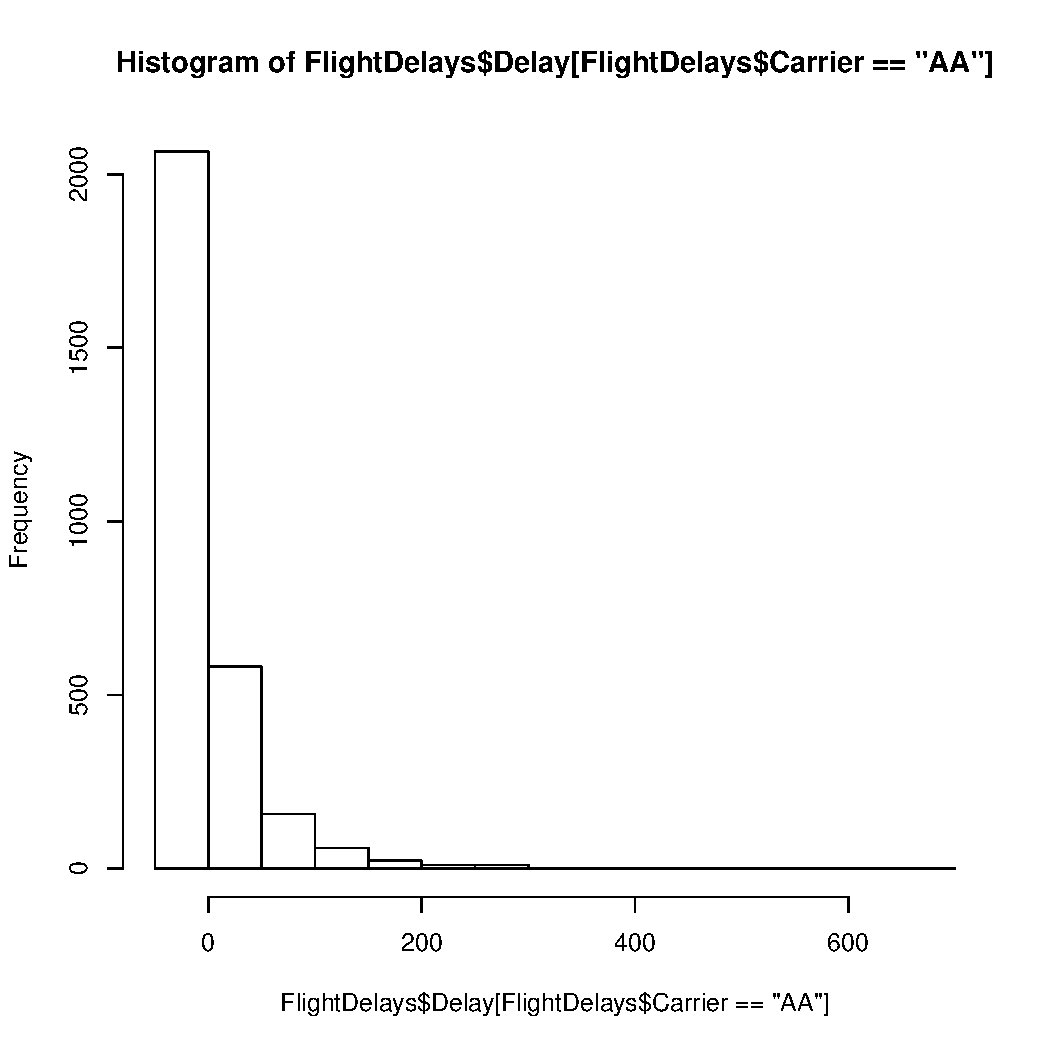
\includegraphics[width=0.33\linewidth]{figure/unnamed-chunk-26-2} 
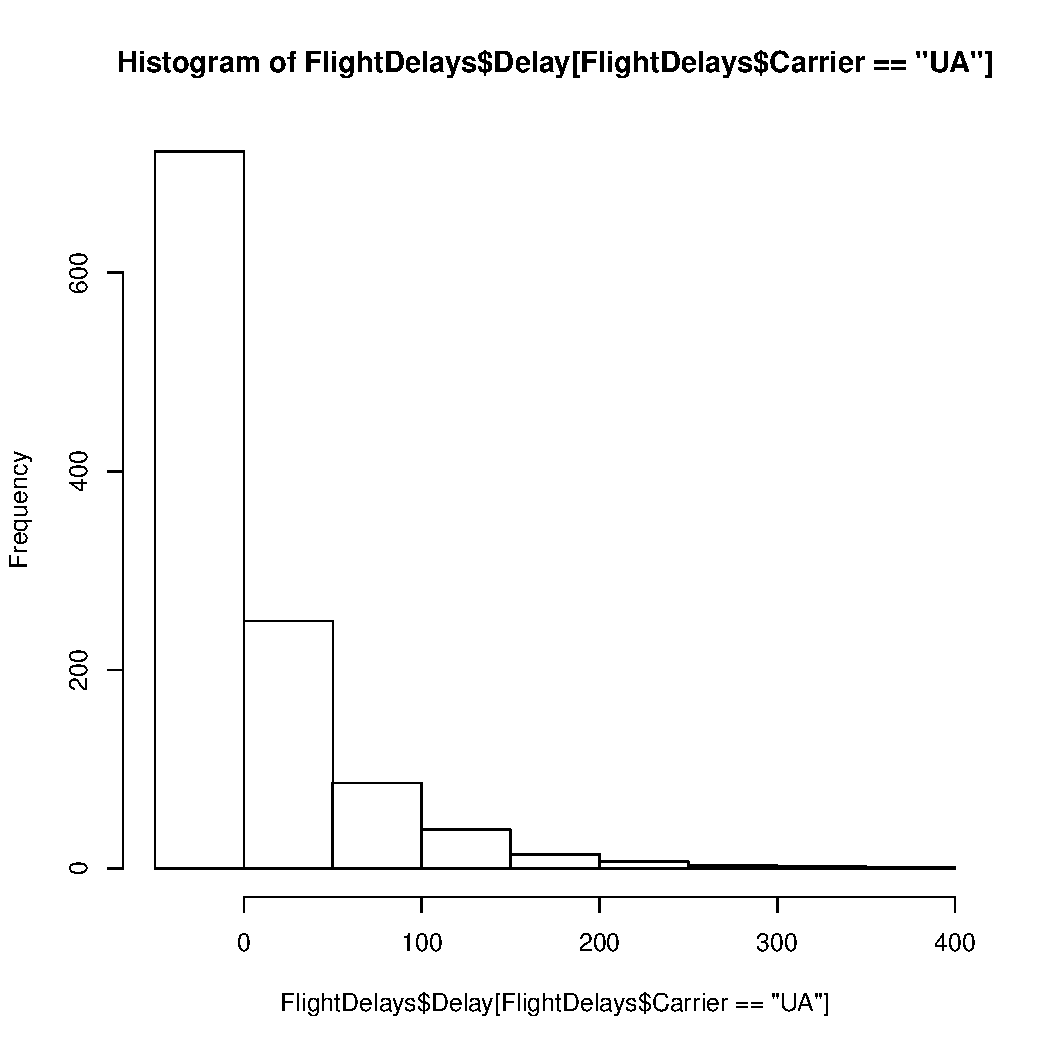
\includegraphics[width=0.33\linewidth]{figure/unnamed-chunk-26-3} 
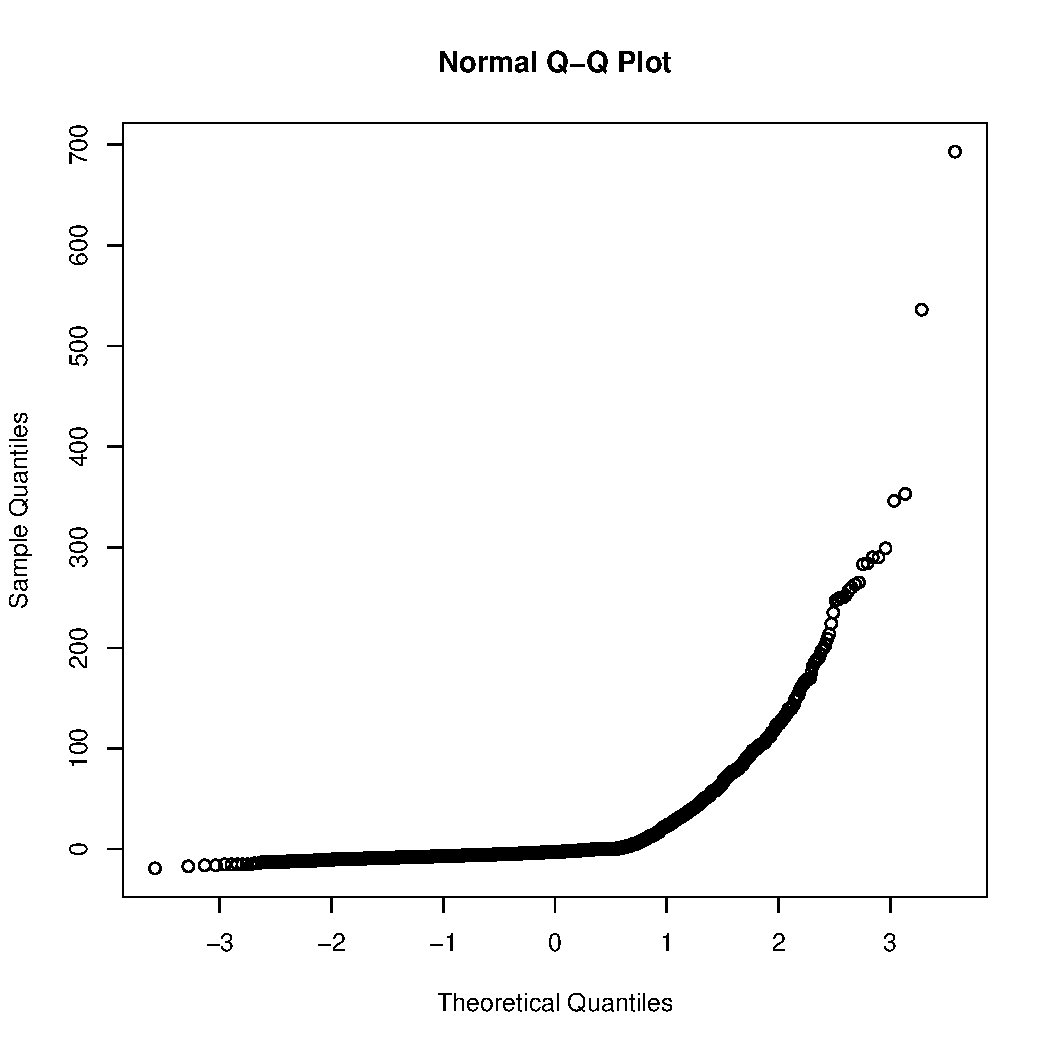
\includegraphics[width=0.33\linewidth]{figure/unnamed-chunk-26-4} 
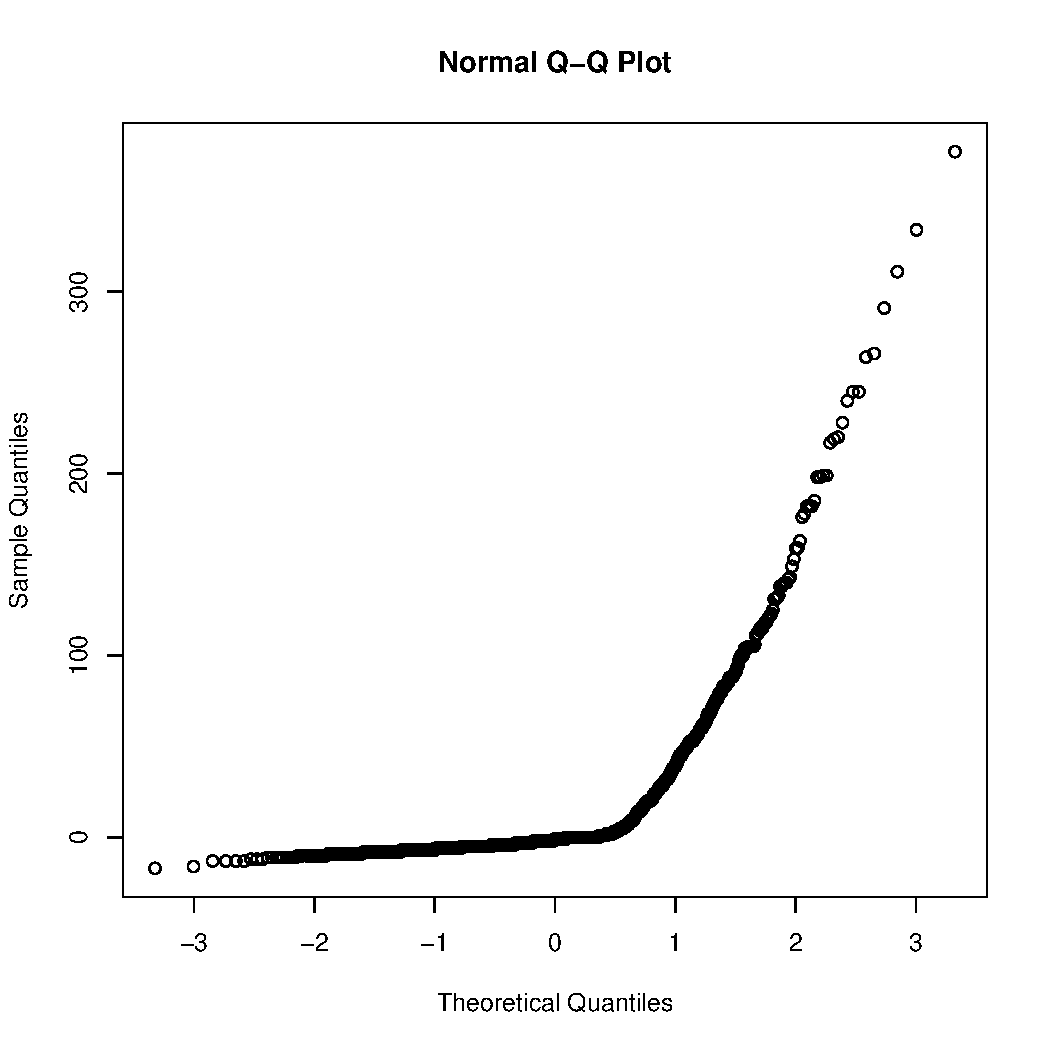
\includegraphics[width=0.33\linewidth]{figure/unnamed-chunk-26-5} 

\end{knitrout}
From the boxplot, both airlines have a significant amount of upper outliers. However the outliers from AA are further out. From the histogram, it seems that the delays follow for each of the airlines follow poisson distributions. The QQnorm plots concur that the distributions are not normal, but the two airlines follow the same distribtuion. 
\subsection*{Part B}
\begin{knitrout}
\definecolor{shadecolor}{rgb}{1, 1, 1}\color{fgcolor}\begin{kframe}
\begin{verbatim}
t.test(FlightDelays$Delay[FlightDelays$Carrier=="AA"], FlightDelays$Delay[FlightDelays$Carrier=="UA"])$conf.int
## [1] -8.903198 -2.868194
## attr(,"conf.level")
## [1] 0.95
aa = FlightDelays$Delay[FlightDelays$Carrier=="AA"]
ua = FlightDelays$Delay[FlightDelays$Carrier=="UA"]
BootstrapMedianDifference = replicate(10000,
                                      median(sample(aa, length(aa),replace = T))-
                                        median(sample(ua, length(ua), replace = T)))

quantile(BootstrapMedianDifference, c(0.025,0.975))
##  2.5% 97.5% 
##    -2    -1
\end{verbatim}
\end{kframe}
\end{knitrout}

The two tests seem to contradict one another because the upper bound of the t test is greater the confidence interval of the mean. This is due to the confidence interval being based on the difference in median whereas the t test is based on the difference in mean. 
\end{document}
